\documentclass[11pt,oneside]{book}
\usepackage{hyperref}
\usepackage{graphicx}
\usepackage{listings}
\usepackage{color}
\usepackage{tikz}
\usepackage[margin=1in]{geometry}
\usepackage{titlesec}
\usepackage{tcolorbox}
\usepackage{fancyhdr}
\usepackage{enumitem}

\titleformat{\chapter}{\normalfont\huge\bfseries}{\thechapter}{20pt}{\huge}
\titlespacing*{\chapter}{0pt}{-30pt}{20pt}

\pagestyle{fancy}
\fancyhf{}
\fancyhead[R]{\leftmark}
\fancyfoot[C]{\thepage}

\title{
    \Huge AP Computer Science Principles\\
    \Large Unofficial Summary\\[0.5em]
    \normalsize\textcolor{red}{Work in Progress - Under Development}
}
\author{\href{https://rowi.dev/}{Robin Wiethüchter}}
\date{\today}

\begin{document}
\maketitle

\begin{tcolorbox}[
    title=Disclaimer,
    colback=white,
    colframe=black,
    width=\textwidth-2cm,
    center
]
This is an \textit{unofficial} study resource not affiliated with College Board\textsuperscript{\textregistered} or Code.org\textsuperscript{\textregistered}. The content may:
\begin{itemize}[leftmargin=*,noitemsep]
    \item Contain errors or inaccuracies
    \item Deviate from official AP\textsuperscript{\textregistered} curriculum guidelines
    \item Not fully align with current exam requirements
    \item Be incomplete or outdated
\end{itemize}
Users should refer to official College Board\textsuperscript{\textregistered} materials for authoritative information.
\end{tcolorbox}

\tableofcontents

\chapter{Digital Information}

\section*{Overview}
Computers can only understand binary - sequences of 0s and 1s. Everything we see and do on computers, from text to images to programs, is ultimately stored and processed as binary data.

\section{Binary and Data Representation}
\begin{itemize}
    \item \textbf{Binary}: A single binary digit (0 or 1) is called a bit. It represents one of two possible states: on/off, true/false, or high/low voltage
    \item \textbf{Bits and Bytes}: 8 bits group together to form 1 byte. This gives us 256 possible unique values ($2^8$). For example, the numbers 0-255 can be stored in one byte
\end{itemize}

\begin{figure}[h]
    \centering
    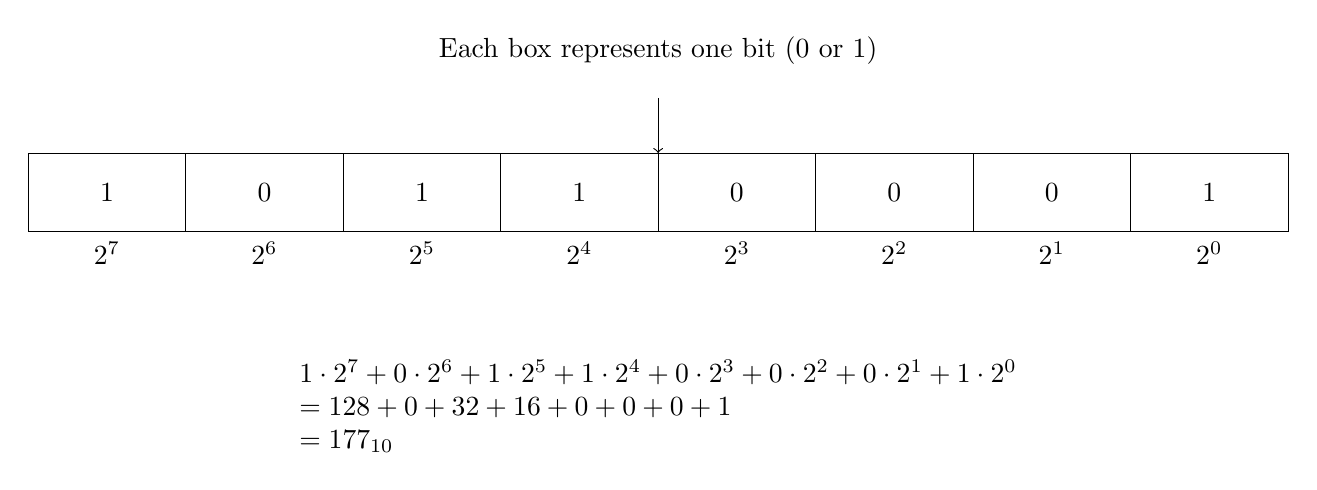
\begin{tikzpicture}[
        box/.style={
            draw,
            rectangle,
            minimum width=2cm,
            minimum height=1cm,
            align=center
        }
    ]
        % Binary representation boxes
        \foreach \x/\v in {0/1,1/0,2/1,3/1,4/0,5/0,6/0,7/1} {
            \node[box] at (\x*2,0) {\v};
        }
        
        % Labels
        \node[above] at (7,1.5) {Each box represents one bit (0 or 1)};
        \draw[->] (7,1.2) -- (7,0.5);
        
        % Power labels below
        \foreach \x/\p in {0/7,1/6,2/5,3/4,4/3,5/2,6/1,7/0} {
            \node[below] at (\x*2,-0.5) {$2^\p$};
        }
        
        % Add calculation below
        \node[below, align=left] at (7,-2) {
            $1 \cdot 2^7 + 0 \cdot 2^6 + 1 \cdot 2^5 + 1 \cdot 2^4 + 0 \cdot 2^3 + 0 \cdot 2^2 + 0 \cdot 2^1 + 1 \cdot 2^0$\\
            $= 128 + 0 + 32 + 16 + 0 + 0 + 0 + 1$\\
            $= 177_{10}$
        };
    \end{tikzpicture}
    \caption{Converting binary to decimal: Each 1 or 0 is multiplied by its position value (powers of 2), then added together}
    \label{fig:binary-byte}
\end{figure}

\section{Number Systems}
\begin{itemize}
    \item \textbf{Binary to Decimal}: To convert binary to decimal, multiply each digit by its position value (powers of 2) and add. For example, $1101_2 = 8 + 4 + 0 + 1 = 13_{10}$
    \item \textbf{Binary Addition}: Add columns right to left, carrying over a 1 when sum exceeds 1. Example:\\
    \hspace{1cm}  1 1 0 1\\
    \hspace{1cm}+ 0 1 1 1\\
    \hspace{1cm}= 1 0 1 0 0
    \item \textbf{Negative Numbers}: Use "two's complement" to represent negatives. Flip bits and add 1. Example: $5_{10} = 0101_2$, $-5_{10} = 1011_2$.
\end{itemize}

\section{Text and Media}
\begin{itemize}
    \item \textbf{Text}: ASCII assigns each character a number from 0-127. 'A' is 65, 'B' is 66, etc. So 'CAT' in binary would be 01000011 01000001 01010100
    \item \textbf{Images}: Pictures are grids of pixels. Each pixel stores RGB (Red, Green, Blue) values from 0-255. More pixels = higher resolution but larger file size
    \item \textbf{Sound}: Sound waves are measured thousands of times per second. Each measurement becomes a number representing the wave's height at that moment
\end{itemize}

\section{Storage and Data Transfer}
\begin{itemize}
    \item \textbf{File Sizes}: As files get bigger, we use larger units: 1 KB = 1,024 bytes, 1 MB = 1,024 KB, 1 GB = 1,024 MB. A typical photo might be 3 MB
    \item \textbf{Data Transfer}: Data moves in packets across networks. Transfer speed depends on bandwidth (capacity) and latency (delay). A slow connection might transfer 1 MB/second
    \item \textbf{Metadata}: Files carry extra information like creation date and size. For example, a photo includes when it was taken, camera settings, and location
\end{itemize}

\section{Programs and Data}
\begin{itemize}
    \item \textbf{Programs}: Software is just a sequence of binary instructions telling the computer what to do. Each instruction might be "add these numbers" or "display this text"
    \item \textbf{Data}: Programs process data - the actual content like your documents, photos, or game saves. The same program can work with different data
    \item \textbf{Compression}: Files can be made smaller by finding and removing patterns. Like writing "123123123" as "123×3". This saves storage space and transfer time
\end{itemize}
\chapter{The Internet}

\section*{Overview}
Exploration of Internet architecture, protocols, and its profound impact on modern society, including cultural, political, and economic implications.

% Key topics:
% - Network protocols
% - Internet architecture
% - Societal impacts 
\chapter{Intro to App Design}

\section*{Overview}
Introduction to fundamental programming concepts through app development, emphasizing collaborative development practices and basic software design principles.

% Key topics:
% - Basic programming concepts
% - Software development lifecycle
% - Collaboration tools and practices 
\chapter{Variables, Conditionals, and Functions}

\section*{Overview}
Core programming constructs that enable data storage, decision-making, and code organization, with emphasis on practical application in app development.

% Key topics:
% - Variable types and scope
% - Control structures
% - Function definition and usage 
\chapter{Lists, Loops, and Traversals}

\section*{Overview}
Working with collections of data, implementing iteration, and processing data sequences to create more sophisticated applications.

% Key topics:
% - Data structures
% - Iteration methods
% - Data processing techniques 
\chapter{Algorithms}

\section*{Overview}
Study of algorithm design, analysis, and evaluation, focusing on efficiency and problem-solving strategies.

% Key topics:
% - Algorithm analysis
% - Complexity considerations
% - Problem-solving approaches 
\chapter{Parameters, Return, and Libraries}

\section*{Overview}
Advanced programming concepts focusing on code reusability, modularity, and the use of external libraries.

% Key topics:
% - Function parameters
% - Return values
% - Library integration 
\chapter{Create PT Prep}

\section*{Overview}
Preparation and practice for the Create Performance Task, focusing on project development and documentation.

% Key topics:
% - Project planning
% - Implementation
% - Documentation requirements 
\chapter{Data}

\section*{Overview}
Exploration of data analysis and visualization techniques, using real-world datasets to discover patterns and draw conclusions.

% Key topics:
% - Data analysis methods
% - Visualization techniques
% - Pattern recognition 
\chapter{Cybersecurity and Global Impacts}

\section*{Overview}
Examination of cybersecurity principles and the broader implications of computing on society, including ethical considerations and policy impacts.

% Key topics:
% - Security principles
% - Ethics in computing
% - Social responsibility 

\bibliographystyle{plain}
\bibliography{references}

\end{document} 